%%\textbf{}%%%%%%%%%%%%%%%%%%%%%%%%%%%%%%%%%%%%%%%%%%%%%%%%%%%%%%%%%%%%%%%%%%%%%%%%%%%%%%
%2345678901234567890123456789012345678901234567890123456789012345678901234567890
%        1         2         3         4         5         6         7         8
% THESIS CHAPTER


\chapter{Other Algorithms for Object Detection}
\label{chap:AppendixVision}
\ifpdf
    \graphicspath{{Vision/Figures/PNG/}{Vision/Figures/PDF/}{Vision/Figures/}}
\else
    \graphicspath{{Vision/Figures/EPS/}{Vision/Figures/}}
\fi

During the simulations, several trials have been done to find a suitable algorithm for the detection of the hole structure. In Chapter \ref{chap:vision} two methods have been discussed as the successful ones. In this appendix, others that have been discarded are briefly presented. Even if they are not used in the last versions of experiments, they can be useful for other purposes, such as detection of other kind of shapes.\\
Each algorithm is taken from OpenCV Detection tutorials (\url{https://docs.opencv.org/3.4/d9/d97/tutorial_table_of_content_features2d.html}), where also other interesting methods can be found.

\section{Corner Detection with the Shi-Harris Method}

\begin{figure}[H]
	\centering
	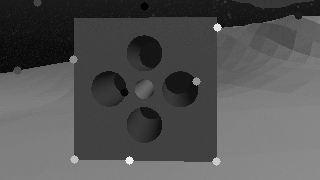
\includegraphics[width=8.0cm]{goodFeatToTrack}
	\caption[Result of \textit{goodFeaturesToTrack()}]{\textit{goodFeaturesToTrack()} result. Only two detected points are the real corners, and the upper ones are not detected.} 
	\label{fig:goodFeatToTrack}
\end{figure}


Following the tutorial (\url{https://docs.opencv.org/3.4.6/d8/dd8/tutorial_good_features_to_track.html}), it has been implemented a corner detector with the Shi-Harris method [\cite{Shi94goodfeatures}] using the OpenCV function \href{https://docs.opencv.org/3.4.6/dd/d1a/group__imgproc__feature.html#ga1d6bb77486c8f92d79c8793ad995d541}{goodFeaturesToTrack()}.\\
This function, in our case, can be useful to find the corners of the hole structure, which is the necessary initialization for the Tracking method used after (section \ref{sec:visDetect}).\\

The original example lets change the number of maximum points to be found. This is useful to reduce the number of false positive corners. The main problem is that the real corners of the square are not the "best" ones. So we can't simply put this parameter equal to 4. On the other side, with a large number of points, would be then difficult to discriminate the right corners from the others.\\
Other interesting parameters are:
\begin{itemize}
	\item \textbf{minDistance}. The minimum distance among the corners to be found.
	\item \textbf{qualityLevel}. A parameter which characterizes the minimum accepted quality of image corners.
	\item \textbf{blockSize}. Size of an average block for computing a derivative covariance matrix over each pixel's neighbourhood.
	\item \textbf{mask}. To specify a certain region of interest in the image. In such a way, corners are searched only in this region. The problem in our case is that without prior works we can't know where the interesting region is (i.e. the region which contains the hole).
\end{itemize}
The points detected are effectively good feature points (as can be seen in figure \ref{fig:goodFeatToTrack}). But, the best ones are not the ones that we want to detect (i.e., the corner of the square).\\
This method should be used as a low level algorithm, to then help higher level ones. For example, to construct some polygons and to check if these polygons are square/rectangles. However, to follow this direction should be better to start from the edges (as done in section \ref{subsec:findSquare}).\\
  
\section{Canny Edge and Hough Transform}
\label{sec:HoughTrasf}
%https://docs.opencv.org/3.4/d9/db0/tutorial_hough_lines.html

\begin{figure}[H]
	\centering
	\centerline{
		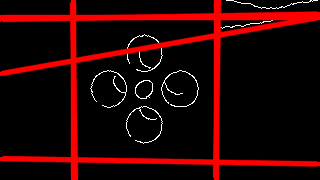
\includegraphics[width=7.0cm]{canny_HoughStandard}
		\qquad
		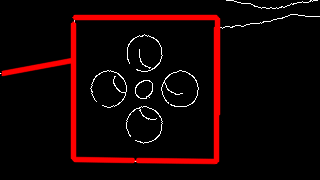
\includegraphics[width=7.0cm]{canny_HoughProb}
	}
	\caption[Results of the Standard Hough Transform and the Probabilistic one]{Results of the Hough Standard Transform (left) and the Probabilistic one (right). In white they are depicted all the edges detected with Canny; the red lines are the detected straight lines, outputs of the method.}
	\label{fig:HoughStandard}
\end{figure}

The Hough Transform [\cite{DudaHoughTrasf}] is a method to detect straight lines in an image. Usually, a preprocessing of the image with an edge detector is used to improve the results, for example with a Canny Edge Detector [\cite{CannyEdge}].\\

The OpenCV tutorial (\url{https://docs.opencv.org/3.4/d9/db0/tutorial_hough_lines.html}) makes use of two types of Hough Transform: the standard \href{https://docs.opencv.org/3.4/dd/d1a/group__imgproc__feature.html#ga46b4e588934f6c8dfd509cc6e0e4545a}{\textit{HoughLines()}} and the probabilistic \href{https://docs.opencv.org/3.4/dd/d1a/group__imgproc__feature.html#ga8618180a5948286384e3b7ca02f6feeb}{\textit{HoughLinesP()}} [\cite{houghprob}].\\
Results are visible in figure \ref{fig:HoughStandard}. The results on the right shows that the probabilistic version is good to detect the square structure of the hole. 
Thus, this method can be used as a good preliminary step to then extract the corner from the detected square.

\newpage
\section{Bounding Box Detection}
\label{sec:boundingBox}
%https://docs.opencv.org/3.4.6/de/d62/tutorial_bounding_rotated_ellipses.html	

\begin{figure}[H]
	\centering
	\centerline{
	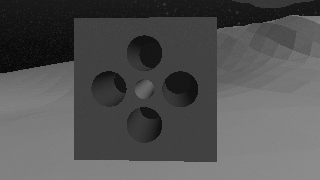
\includegraphics[width=7.0cm]{BoundBox_sourceOnlyPolig}
	\qquad
	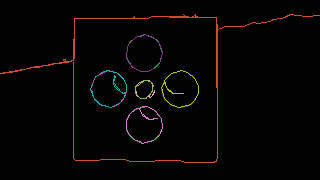
\includegraphics[width=7.0cm]{BoundBox_resultOnlyPolig}
	}
	\caption[Result of \emph{findContours()}]{Result of \emph{findContours()}: on the left the original image, on the right the contours detected.}
	\label{fig:BoundBoxresultOnlyPolig}
\end{figure}

\begin{figure}[H]
	\centering
	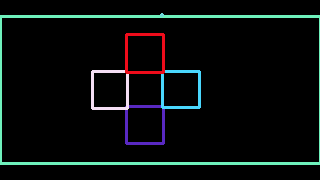
\includegraphics[width=7.0cm]{BoundBox_resultOnlyRect}
	\caption[Result of Bounding Box detection]{Result of Bounding Box detection, where they are visible the drawn bounding boxes around the holes.}
	\label{fig:BoundBoxresultOnlyRect}
\end{figure}

The code derived from an OpenCV tutorial (\url{https://docs.opencv.org/3.4.6/de/d62/tutorial_bounding_rotated_ellipses.html}).\\
First, a Canny edge detector is used to preprocess the image. Then, the function \href{https://docs.opencv.org/3.4.6/d3/dc0/group__imgproc__shape.html#ga17ed9f5d79ae97bd4c7cf18403e1689a}{\textit{findContours()}} is called to retrieve contours with the algorithm described in \cite{findcountors}. As can be noticed, these initial steps are the same of the implemented method of section \ref{subsec:findSquare}. The difference in this tutorial is that, after these passages, bounding boxes are drawn around some particular shapes detected.\\

The result after the first step is shown in figure \ref{fig:BoundBoxresultOnlyPolig}. We can see that this passage already reveals the square, that is important for the method described in \mbox{section \ref{subsec:findSquare}.}\\
Instead, the algorithm presented here continues in a different direction, which brings us to the final result of figure \ref{fig:BoundBoxresultOnlyRect}.\\

This tutorial is recalled because it can be useful to find other kinds of shapes, for example an hole structure which is not a rectangle or a square.


\section{2D Feature Matching \& Homography}
%https://docs.opencv.org/3.4/d7/dff/tutorial_feature_homography.html
\begin{figure}[H]
	\centering
	\centerline{
		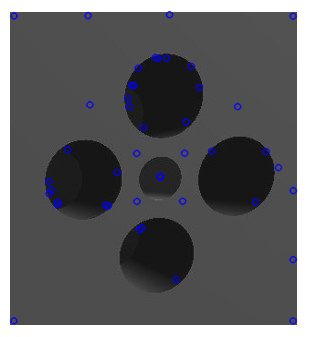
\includegraphics[width=3.8cm]{new_featHomog_SURF_templKeyPoint}
		\qquad
		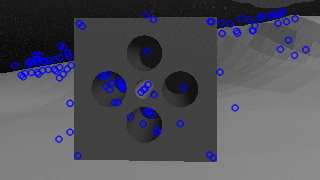
\includegraphics[width=7.1cm]{new_featHomog_SURF_cameraKeyPoint}
	}
	\vspace{10px}
	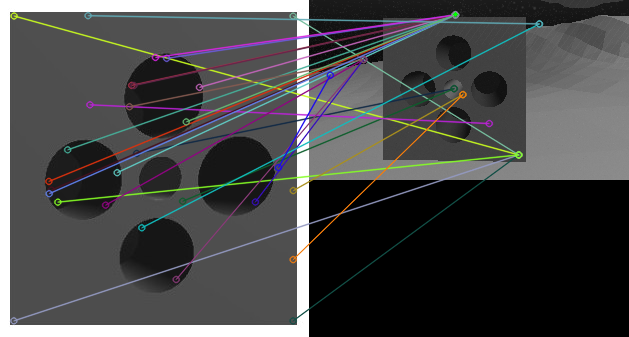
\includegraphics[width=9cm]{new_featHomog_SURF_result}
	\caption[Result of 2D Feature Matching]{Result of the 2D Feature Matching. Above, the blue circles are the detected features in the \textit{object image} (on the left) and in the \textit{scene image} (on the right). Below, the output of the matching passage, which shows clearly a bad outcome.}
	\label{fig:featHomog}
\end{figure}

\textit{Image features} are small patches that are useful to compute similarities between images. These are different from corner points; they indicates particular details that stand out in the image. Detecting these areas is useful to recognize objects of interest, as a sort of \textit{template matching} (please note that this method is not a template matching as the one of section \ref{subsec:templateMatch}).\\
The \textit{descriptors} of these features contain the visual description of the patches, which are used to recognize similarities between different images.\\

This method needs an \textit{object image} and a \textit{scene image}. The first is a sort of template which contains only the object to be found (in this case, the square face of the hole). The second is the image in which we want to detect this object (in this case, what the camera is seeing).\\
After good features are extracted from both images, the \textit{descriptors} are used to \textit{match} them, thus, detecting the object in the scene.
Then, it is necessary to find the perspective transformation between the object image and the scene (i.e. find the homography). This is needed to take into account that usually the pose and the scaling of the object in the scene are not the same of the ones of the object image.\\
The OpenCV tutorial (\url{https://docs.opencv.org/3.4/d7/dff/tutorial_feature_homography.html}) uses different tools:
\begin{itemize}
	\item \textbf{SURF} (Speeded Up Robust Features) Detector [\cite{surfDet}] to extract the features, and to compute the descriptors.
	\item \textbf{FLANN} (Fast Library for Approximate Nearest Neighbors) matcher [\cite{flannMatch}] to match the features of the two images.
	\item \textbf{Lowe's ratio test} [\cite{loweTest}] to take only the best matches.
	\item \textbf{RANSAC} (RANdom SAmple Consensus) [\cite{ransacHomog}] method to find the homography with the function \href{https://docs.opencv.org/3.4/d9/d0c/group__calib3d.html#ga4abc2ece9fab9398f2e560d53c8c9780}{\textit{findHomography()}}.
\end{itemize}

\vspace{20px}
In this case, results are unsatisfactory, as can be seen in figure \ref{fig:featHomog}. The main problem is that in this particular scene there are not nice distinct features. Also, the symmetry of the structure does not help, because there are a lot of particulars that are similar (like the square sides and the holes). As can be seen in the results of the previously cited \href{https://docs.opencv.org/3.4/d7/dff/tutorial_feature_homography.html}{tutorial}, good outcomes are obtained for food boxes. In fact, this method is often exploited for scenes where a lot of details are present (e.g. graffiti painting, supermarket shelf). In underwater cases, realistic infrastructures have not so many details, and so also the simulated scenario of this thesis.\\

There are a lot of parameters to set for the three main tools (SURF, FLANN, and RANSAC). Various options have been tried but no-one was satisfactory. Also, different detectors (like SWIFT [\cite{loweTest}]) and matchers (like Brute-Force), have been tried, again with poor results.\\
Anyway, the variety of tools and parameters makes this method suitable for a lot of applications, and it should be taken into consideration in other applications.






